% Appendix A

\chapter{Thalamic Drive of Cortical Parvalbumin-Positive Interneurons during Down States in Anesthetized Mice} % Main appendix title
\label{paper_pasquale} % For referencing this appendix elsewhere, use \ref{AppendixA}
In the study presented in Appendix A, I was responsible for the analysis of Local Field Potential (LFP) recordings in anesthetized mice (Figure 4).
I developed the algorithm for detection of slow waves and up and down states in the LFP measurements (Supplementary Figure 4). 
I measured the latency of down-to-up state transitions after optogenetic inhibitory manipulation of Parvalvumin postive interneurons under control condition and after silencing the thalamus via muscimol injection (Figure 4).
I also used a Linear Mixed Effects model to study the interaction between pharmacological (muscimol) treatment and optogenetic stimulation in slow waves transitions (Figure 4). 

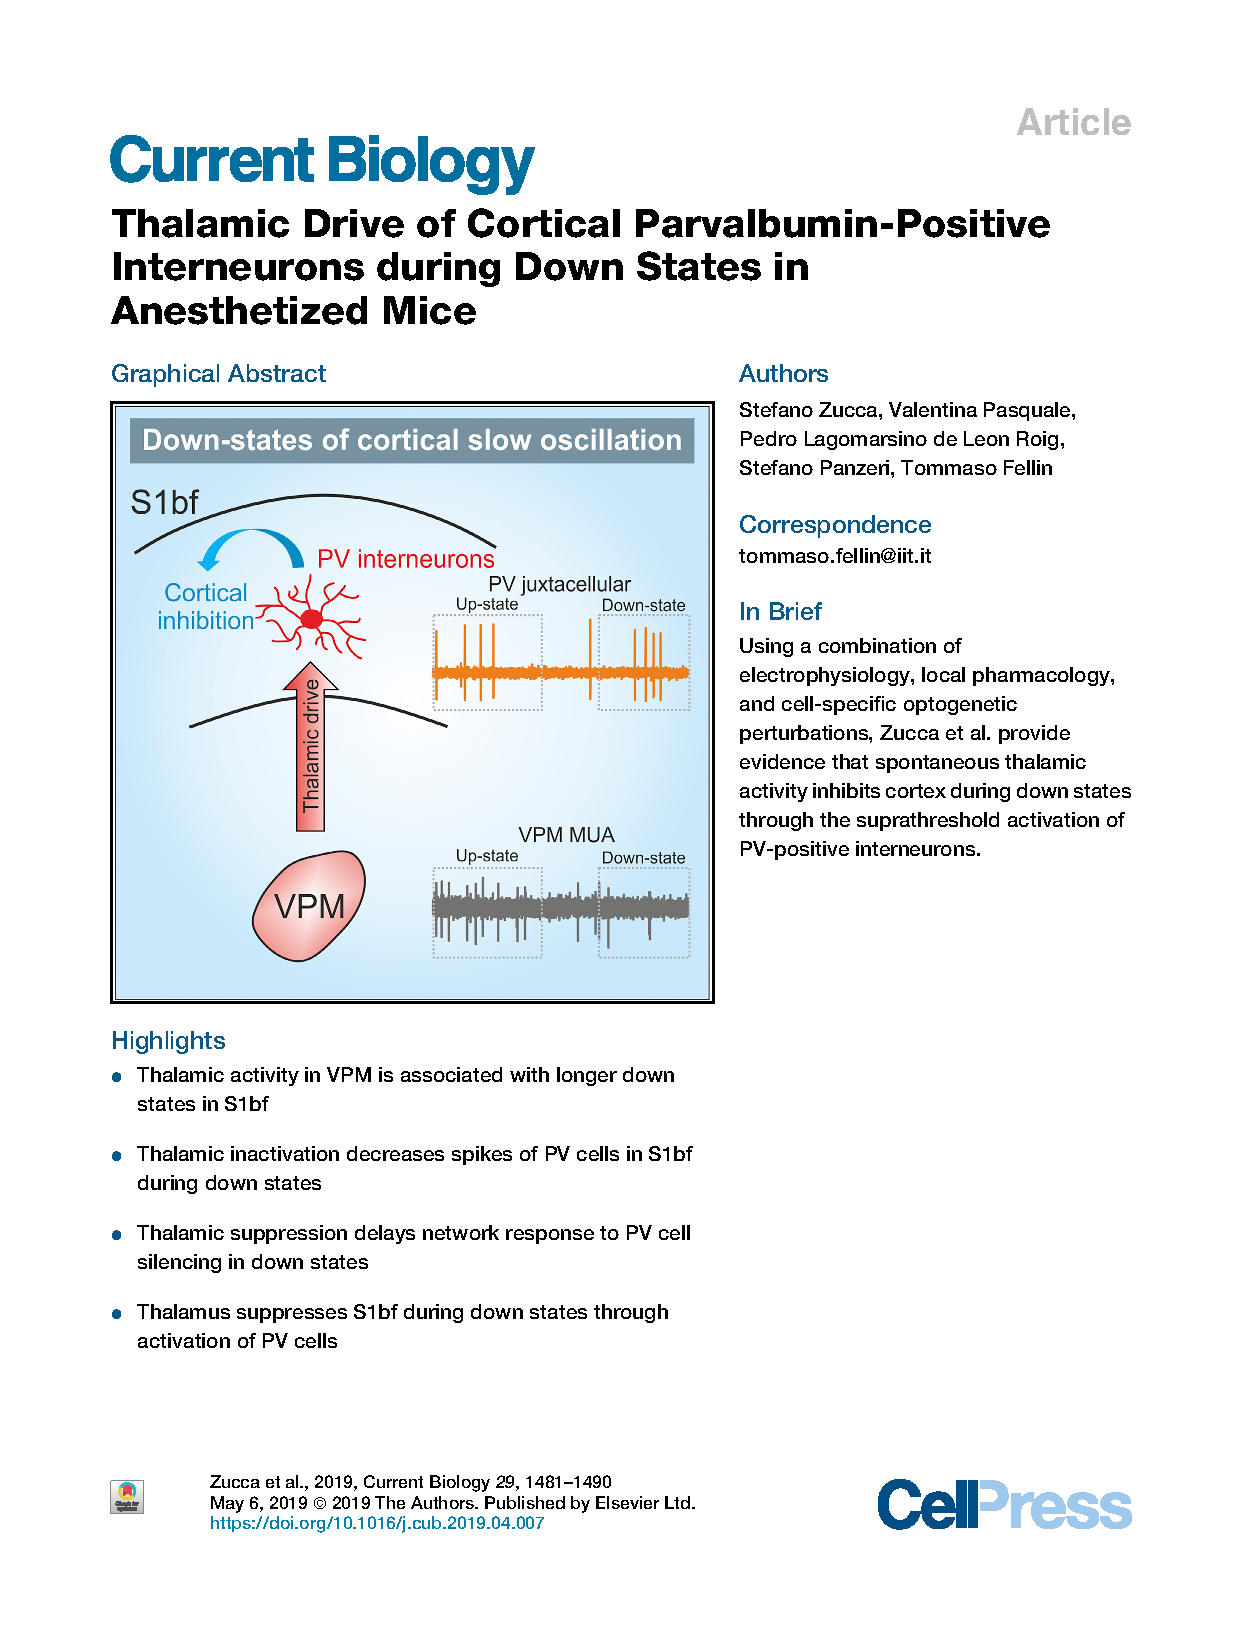
\includepdf[pages=-,pagecommand={\thispagestyle{plain}}]{pasquale_paper.pdf}
